\documentclass[12pt]{article}

\usepackage{graphicx}

\begin{document}
\linespread{1.0}
\begin{titlepage}
	\begin{center}
		\large{University of Puerto Rico\\
			Mayagüez Campus\\
			\vspace{\baselineskip}
			Department of Electrical and Computer Engineering}\\
		\vspace{5\baselineskip}
		\Huge{\underline{M.O.S.I.S U.I 2.0 Progress Report}\\}
		\vspace{\baselineskip}
		\large by\\
		Fabio J. Matos Nieves\\
		Eduardo S. Miranda Figueroa\\
		\normalsize
		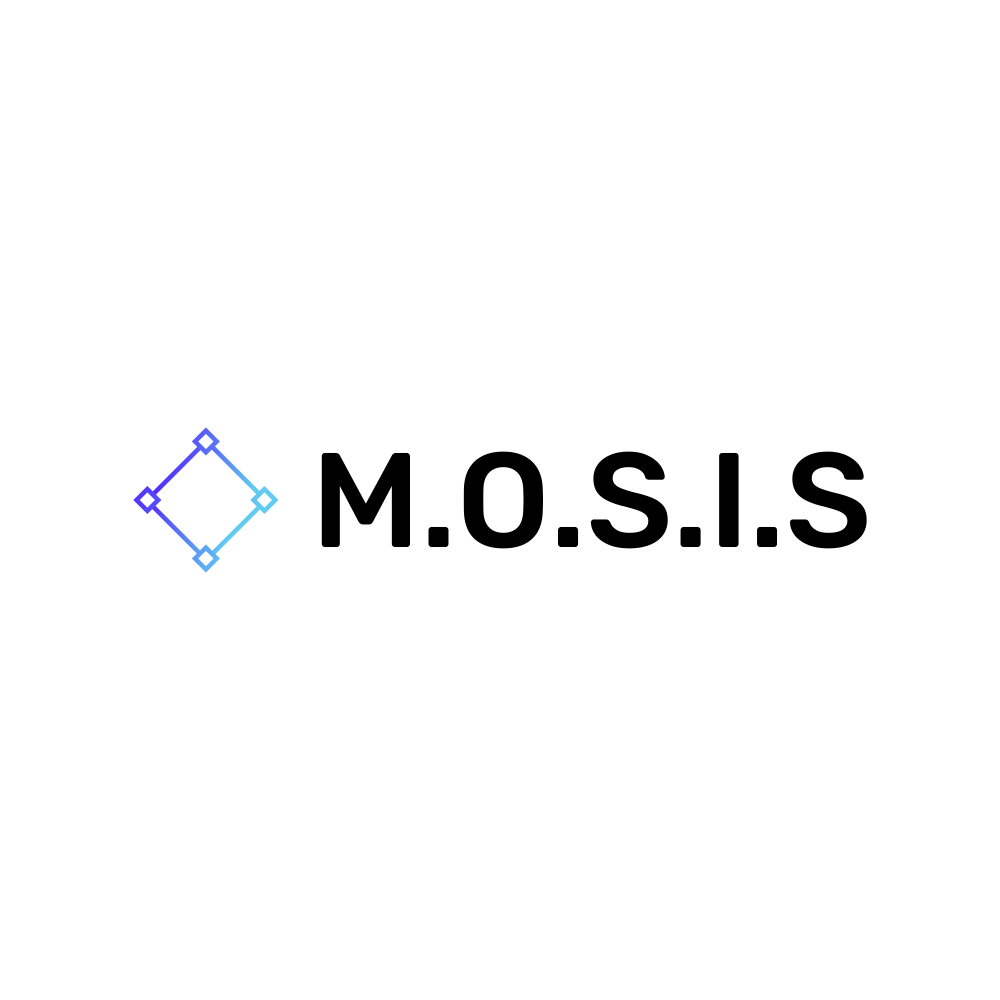
\includegraphics[scale=0.15]{../../M.O.S.I.S Logo/default.png}\\
		\vspace{4\baselineskip}
		\large
		For: Nayda Santiago\\
		Course: ICOM 5047, section 016\\
		Date: September 14, 2023\\
		\normalsize

	\end{center}
\end{titlepage}
\section*{Executive Summary}
\tableofcontents
\section{Introduction}
The Marine Operated Stereoscopic Imaging System (M.O.S.I.S) is a device created by David M. Repollet Otero along with Manuel A. Jimenez Cedeno in order to study marine life \textit{in situ} in stereoscopic vision while capturing environmental conditions such as temperature, pH, pressure and dissolved oxygen. As of November 27, 2023, the microscope itself has a fully completed user interface capable of capturing various kinds of still photography and videos. However, at its core, the M.O.S.I.S microscope is an embedded system running a Raspberry Pi 4b, meaning that processing speed and memory are both severely limited. But not only is processing power limited, but the device itself will be deployed in an extremely hostile environment, where the microscope can be destroyed at a moments notice. Even more so, the microscope does not provide the means to recover the captured data nor does it provide the means to analyses and present the data to the user. The host software for the M.O.S.I.S microscope aims to backup the data captured by the M.O.S.I.S microscope, analyses the data captured by the microscope and generate reports based on the captured data.\\
\subsection{System Requirements}
\subsubsection{Domain Requirements}
\begin{itemize}
	\item The system-to-be must allow the backup of the M.O.S.I.S project Raspberry Pi's operating system.
	\item The system-to-be must allow the backup of the images captured by the M.O.S.I.S microscope Raspberry Pi.
	\item The system-to-be must have a database that stores the media captured by the M.O.S.I.S microscope Raspberry Pi.
	\item The system-to-be must have a database that stores the sensor data captured by the M.O.S.I.S microscope Raspberry Pi.
	\item The system-to-be must create a stereoscopic image from the media captured by the M.O.S.I.S microscope Raspberry Pi.
	\item The system-to-be must have the means to pre-configured the type of media capture before deployment in the field.
	\item The system-to-be must tag the media captured the M.O.S.I.S Raspberry Pi with the information stored in the database.
	\item The system-to-be must analyze the captured media for bleaching estimates.
	\item The system-to-be must create reports from the captured media.
\end{itemize}
\subsubsection{Interface Requirements}
\begin{itemize}
	\item The system-to-be's database must contain image information that includes:
	      \begin{itemize}
		      \item Left Camera Image
		      \item Right Camera Image
		      \item Stereoscopic Image
		      \item Left Threshold Image
		      \item Right Threshold Image
		      \item Time Stamp
		      \item Temperature
		      \item Ph
		      \item Pressure
		      \item Dissolved Oxygen (DO) Content
	      \end{itemize}
	\item The system-to-be must have a home page where there is a preview of all images currently within the database.
	\item The system-to-be must create an individual page for each entry within the database.
\end{itemize}
\section{Design Criteria and Specifications}
\subsection{System Specifications}
\begin{itemize}
	\item Backs up M.O.S.I.S microscope media data via SSH
	\item Generates stereoscopic images or video from left and right cameras.
	\item Tags stereoscopic media with the sensor data and time stamp associated with that entry.
	\item Generate threshold images from captured media.
	\item Allows searching by ID, shot type, illumination type and date.
	\item Exports either whole database or searched media entries to a PDF report.
	\item Creates compressed backups of M.O.S.I.S microscope operating system.
	\item Officially supports Windows and Linux operating systems.
\end{itemize}
\subsection{Design Criteria}
The main design criterion for the host software was to create a set of user friendly utilities that:
\begin{itemize}
	\item Abstract and automates the process of interacting with the M.O.S.I.S microscope as much as possible.
	\item Is usable by marine biologist end users.
	\item Is reliable enough to backup and analyze the data from the M.O.S.I.S microscope for the lifetime of the device
	\item Is free and open source.
\end{itemize}
These design criteria are in part due to the target users of the M.O.S.I.S microscope, those being, marine biologist researchers. These researchers know how to analyze the captured data and to draw conclusions from said data, but most of them lack the expertise to use complex computer software, especially ones designed for computer scientists and engineers. Thus, with these design criterion in mind, the host software design process was applied in the following ways:
\begin{enumerate}
	\item Minimize interaction with the command line as much as possible.
	\item Automate the installation of dependencies as much as possible.
	\item Web browser based.
	\item Streamline the process of backing up the captured media and microscope operating system.
	\item Friendly and modern user interface design.
	\item Automate the process of data analysis.
	\item Streamline the process of data export.
	\item Seamless integration between the host machine and the Raspberry Pi.
\end{enumerate}
\subsection{Analysis of alternatives}
\section{Methods and approach to the solution}
\section{Results, and impact of the project}
\section{Conclusions and Future Work}
\bibliographystyle{IEEEtranN}
\addcontentsline{toc}{section}{Bibliographic References}
\bibliography{../../../../References_Library/ICOM5047}
\appendix
\section{Glossary}
\section{User Requirements}
\section{System Specifications}
\section{Analysis of Alternatives}
\section{System Architecture and Interfaces}
\section{Design Documentation}
\section{Testing Plan}
\section{Task Progress and Gantt Chart}
\end{document}